
\documentclass{standalone}
\usepackage{tikz}
\begin{document}
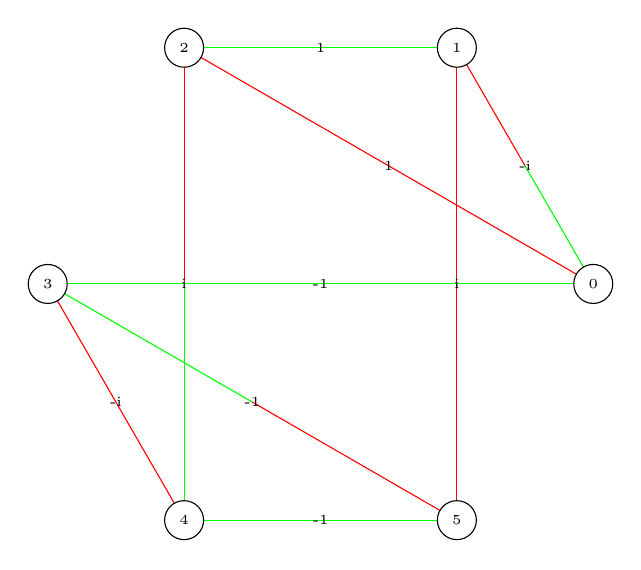
\begin{tikzpicture}
\tikzstyle{every node}=[font=\tiny]
\draw [style=thin, color=green] (3.4641016151377553,0.0) to (2.598076211353317,1.5000000000000002);
\draw [style=thin, color=red] (2.598076211353317,1.5000000000000002) to (1.732050807568878,3.0000000000000004);
\node [style=circle, draw=none] at (2.598076211353317,1.5000000000000002) {-i};
\draw [style=thin, color=red] (3.4641016151377553,0.0) to (0.8660254037844392,1.5000000000000004);
\draw [style=thin, color=red] (0.8660254037844392,1.5000000000000004) to (-1.732050807568877,3.000000000000001);
\node [style=circle, draw=none] at (0.8660254037844392,1.5000000000000004) {1};
\draw [style=thin, color=green] (3.4641016151377553,0.0) to (0.0,2.1211504774498143e-16);
\draw [style=thin, color=green] (0.0,2.1211504774498143e-16) to (-3.4641016151377553,4.2423009548996286e-16);
\node [style=circle, draw=none] at (0.0,2.1211504774498143e-16) {-1};
\draw [style=thin, color=green] (1.732050807568878,3.0000000000000004) to (5.551115123125783e-16,3.000000000000001);
\draw [style=thin, color=green] (5.551115123125783e-16,3.000000000000001) to (-1.732050807568877,3.000000000000001);
\node [style=circle, draw=none] at (5.551115123125783e-16,3.000000000000001) {1};
\draw [style=thin, color=red] (1.732050807568878,3.0000000000000004) to (1.7320508075688767,-6.661338147750939e-16);
\draw [style=thin, color=red] (1.7320508075688767,-6.661338147750939e-16) to (1.7320508075688754,-3.0000000000000018);
\node [style=circle, draw=none] at (1.7320508075688767,-6.661338147750939e-16) {i};
\draw [style=thin, color=red] (-1.732050807568877,3.000000000000001) to (-1.732050807568878,6.661338147750939e-16);
\draw [style=thin, color=green] (-1.732050807568878,6.661338147750939e-16) to (-1.7320508075688792,-2.9999999999999996);
\node [style=circle, draw=none] at (-1.732050807568878,6.661338147750939e-16) {i};
\draw [style=thin, color=red] (-3.4641016151377553,4.2423009548996286e-16) to (-2.5980762113533173,-1.4999999999999996);
\draw [style=thin, color=red] (-2.5980762113533173,-1.4999999999999996) to (-1.7320508075688792,-2.9999999999999996);
\node [style=circle, draw=none] at (-2.5980762113533173,-1.4999999999999996) {-i};
\draw [style=thin, color=green] (-3.4641016151377553,4.2423009548996286e-16) to (-0.8660254037844399,-1.5000000000000007);
\draw [style=thin, color=red] (-0.8660254037844399,-1.5000000000000007) to (1.7320508075688754,-3.0000000000000018);
\node [style=circle, draw=none] at (-0.8660254037844399,-1.5000000000000007) {-1};
\draw [style=thin, color=green] (-1.7320508075688792,-2.9999999999999996) to (-1.887379141862766e-15,-3.000000000000001);
\draw [style=thin, color=green] (-1.887379141862766e-15,-3.000000000000001) to (1.7320508075688754,-3.0000000000000018);
\node [style=circle, draw=none] at (-1.887379141862766e-15,-3.000000000000001) {-1};
\node [style=circle, fill=white, draw=black] (0) at (3.4641016151377553,0.0) {0};
\node [style=circle, fill=white, draw=black] (1) at (1.732050807568878,3.0000000000000004) {1};
\node [style=circle, fill=white, draw=black] (2) at (-1.732050807568877,3.000000000000001) {2};
\node [style=circle, fill=white, draw=black] (3) at (-3.4641016151377553,4.2423009548996286e-16) {3};
\node [style=circle, fill=white, draw=black] (4) at (-1.7320508075688792,-2.9999999999999996) {4};
\node [style=circle, fill=white, draw=black] (5) at (1.7320508075688754,-3.0000000000000018) {5};
\end{tikzpicture}
\end{document}